\documentclass[conference]{IEEEtran}

\IEEEoverridecommandlockouts

\usepackage{amsmath}
\usepackage{amssymb}
\usepackage{array}
\usepackage{booktabs}
\usepackage{cite}
\usepackage{graphicx}
\usepackage{tikz}
\usepackage{url}
\usepackage{xspace}
\usetikzlibrary{arrows.meta,fit,positioning,shapes.geometric}

\newcommand{\kframework}{K Framework\xspace}
\newcommand{\bitcoin}{Bitcoin\xspace}
\newcommand{\kcell}[1]{\texttt{<#1>}\xspace}

\begin{document}

\title{K-Bitcoin Script: An Executable Semantics for Modern Bitcoin Script}

\author{
  \IEEEauthorblockN{Jeff Zou}
  \IEEEauthorblockA{
    CS 521: Programming Languages and Formal Methods\\
    University of Illinois at Urbana-Champaign\\
    jizezou2@illinois.edu
  }
  \and
  \IEEEauthorblockN{Lawrence Wang}
  \IEEEauthorblockA{
    CS 521: Programming Languages and Formal Methods\\
    University of Illinois at Urbana-Champaign\\
    lw41@illinois.edu
  }
}

\maketitle
\thispagestyle{plain}
\pagestyle{plain}

\begin{abstract}
\bitcoin Script is the consensus-critical stack language used to authorize
transaction inputs.  Although intentionally small, its operational behavior is
distributed across byte-level script decoding, stack evaluation, soft-fork
flags, transaction-dependent signature hashing, witness programs, and
Taproot/Tapscript resource rules.  This report presents K-Bitcoin Script, an
executable and formally verifiable semantics of \bitcoin Script in the
\kframework.  Following the style of prior large K semantics such as KEVM,
KJS, and K-Java, we emphasize the engineering choices needed to make a language
definition simultaneously executable, testable, and useful as a reference
artifact.  The semantics covers legacy, SegWit v0, and Taproot/Tapscript
validation paths, including BIP-143, BIP-341, and BIP-342 signature hashing.
We validate it against Bitcoin Core's script and transaction test vectors, a
mainnet-derived benchmark dataset, and 72 K reachability claims: 70 discharged
by the Haskell Kore prover and two concrete HTLC hash-path claims checked
through the LLVM-backed execution path.  On a 288,190-input dataset, the latest
benchmark run on an Apple M4 Pro produces 288,045 paired K/Core measurements
with zero mismatches; summing the timed per-input verifier medians gives
175.4 seconds for K and 84.2 seconds for \texttt{libbitcoinconsensus}.  We also
report the
project's AI-assisted development methodology: language model agents were used
for implementation and debugging, while Bitcoin Core vectors, BIP vectors,
\texttt{libbitcoinconsensus}, and mainnet replay served as the ground truth.
\end{abstract}

\begin{IEEEkeywords}
Bitcoin Script, formal semantics, K Framework, Taproot, executable semantics,
benchmarking
\end{IEEEkeywords}

\section{Introduction}

\bitcoin consensus depends on faithful validation of each non-coinbase
transaction input.  For common transactions this validation is fast enough to
look routine, but semantically it is dense: the interpreter must decode
minimally encoded byte strings, maintain multiple stacks, enforce soft-fork
flags, compute signature hashes over transaction context, switch execution
phases for P2SH and witness programs, and implement distinct rules for legacy,
SegWit, and Taproot-era spends.  Production implementations such as Bitcoin
Core are authoritative engineering artifacts, but they are not designed to be
mathematical specifications.

The executable-semantics approach taken by the \kframework has been applied to
large real-world languages and machines.  KEVM formalizes the Ethereum Virtual
Machine and evaluates both correctness and performance against the official
Ethereum test suite~\cite{kevm}.  KJS gives an executable semantics for
JavaScript and uses the official ECMAScript conformance suite to test
coverage~\cite{kjs}.  K-Java formalizes Java 1.4 and reports a test-driven
development process with a large conformance suite~\cite{kjava}.  These papers
share a useful pattern: make the semantics executable, define the configuration
and transition rules in K, test the result against external conformance
artifacts, and then demonstrate at least one concrete use of the semantics.

This project follows that pattern for \bitcoin Script.  The goal is not to
replace Bitcoin Core, but to build an independent artifact that is precise
enough to run real inputs, readable enough to audit, and practical enough to
use in regression testing and offline validation.

\subsection{Motivations}

\bitcoin Script is a good target for executable semantics for three reasons.
First, it is consensus-critical: an implementation disagreement can split the
network.  Second, the language is bounded and deterministic for a fixed
transaction context, making it more tractable than general-purpose languages.
Third, Script's historical evolution has produced many small semantic regimes:
pre-P2SH, P2SH, strict DER signatures, locktime and sequence checks, SegWit v0,
and Taproot/Tapscript.  A formal model can expose the phase boundaries and
flag-dependent behavior that are otherwise interleaved in implementation code.

\subsection{Challenges}

The central challenge is that script verification is not just stack-machine
execution.  Signature opcodes require transaction-dependent preimages; those
preimages vary across legacy, BIP-143, BIP-341, and BIP-342 paths.  Witness
programs alter the script being executed and the data committed to by
signatures.  Tapscript changes opcode validity, introduces
\texttt{OP\_CHECKSIGADD}, and accounts for a signature validation budget.

The second challenge is performance.  A semantics that can execute one test
case is not automatically useful on mainnet-sized datasets.  In early honest
benchmarks, K spent most of its time moving large transaction byte strings
through textual KORE and reconstructing large result patterns.  The final
benchmark in this report relies on binary KORE construction, subprocess
chunking, native cryptographic hooks, and a concrete cleanup rule that removes
large no-longer-observed cells from ordinary \texttt{done}-phase final
configurations.

\subsection{Contributions}

This report makes the following contributions.

\begin{itemize}
  \item It describes an executable K semantics for modern \bitcoin Script,
  including legacy, SegWit v0, and Taproot/Tapscript validation phases.
  \item It explains how transaction context, previous outputs, witness data,
  signature hash modes, and consensus flags are represented in the K
  configuration.
  \item It presents 72 K reachability claims, 70 verified by the Haskell Kore
  prover and two concrete HTLC hash-path claims checked with the LLVM-backed
  execution path, covering arithmetic opcode correctness, historical soft-fork
  bug fixes (MINIMALDATA, NULLDUMMY, CLEANSTACK,
  DISCOURAGE\_UPGRADABLE\_NOPS), and flag-sensitive behavioral boundaries.
  \item It reports validation against Bitcoin Core test vectors and a fresh
  mainnet benchmark run on the merged \texttt{main} branch.
  \item It records the AI-assisted, test-driven development process used to
  build the artifact, including the actual model families used and the external
  oracles that constrained them.
  \item It documents the optimization path that reduced the honest K/Core
  performance ratio from 149$\times$ in the first complete run to 2.1$\times$
  on the latest run (Apple M4 Pro, \texttt{libbitcoinconsensus} v27.2).
\end{itemize}

\section{Background}

\subsection{Bitcoin Script}

\bitcoin Script is a stack-based language used to specify spending conditions.
A transaction input provides unlocking data, traditionally a
\texttt{scriptSig}; the previous output provides the locking
\texttt{scriptPubKey}.  Validation executes these programs under consensus
flags determined by block height and transaction context.  P2SH adds a redeem
script phase.  SegWit v0 moves witness data outside the legacy transaction ID
and changes the signature hash algorithm via BIP-143.  Taproot introduces
SegWit version 1 outputs, key-path spends, script-path spends, Schnorr
signatures, and Tapscript validation rules via BIP-341 and BIP-342.

\subsection{The K Framework}

K definitions describe syntax, configurations, and rewrite rules.  From a
definition, K can generate parsers, interpreters, symbolic execution tools, and
proof infrastructure.  The prior K papers use this generated-tool approach as a
methodological constraint: a semantics should be executable, tested against
external programs, and reusable for more than prose documentation.  K-Bitcoin
Script adopts the same constraint.  The repository contains about 5.2 KLOC of
K definition files across modules for decoding, flow control, stack behavior,
arithmetic, cryptography, signature checks, transaction parsing, and sighash
construction.

\section{K Semantics of Bitcoin Script}

This section gives an implementation-oriented overview of the K definition.
The goal is to make the report readable even to a reader who has not opened
the repository.  The definition follows the same discipline used by KEVM, KJS,
and K-Java: the prose explains the organization, but the executable artifact
is the semantics itself.  In this project, that artifact is a collection of K
modules under \texttt{script-semantics/}, backed by native hooks for
cryptographic primitives and by a Python runtime wrapper that constructs the
initial K configuration.

\subsection{Definition Organization}

The executable entry point is \texttt{script.k}.  It imports a core semantics
module and the modules that define decoding, flow control, stack operations,
arithmetic, and signature behavior.  The core module,
\texttt{script-semantics.k}, owns the top-level configuration, phase sort,
failure mechanism, phase transition rules, witness dispatch, and Taproot
verification skeleton.  Supporting modules then define the local rewrite rules
for most opcode families, while the core module still contains a small set of
foundational opcode rules used by common script templates and phase machinery.

Figure~\ref{fig:module-map} shows the dependency shape.  The important point is
that \texttt{script-decode.k} is not merely a parser.  It is part of the
operational semantics: decoding emits K computations such as
\texttt{\#guardExec(OP\_CHECKSIG)} and then recursively schedules decoding of
the remaining byte string.  This makes byte-level consensus checks, such as
push-size limits and Tapscript \texttt{OP\_SUCCESSx}, visible in the same
rewrite system as ordinary stack-machine rules.

\begin{figure*}[t]
  \centering
  \resizebox{\textwidth}{!}{%
  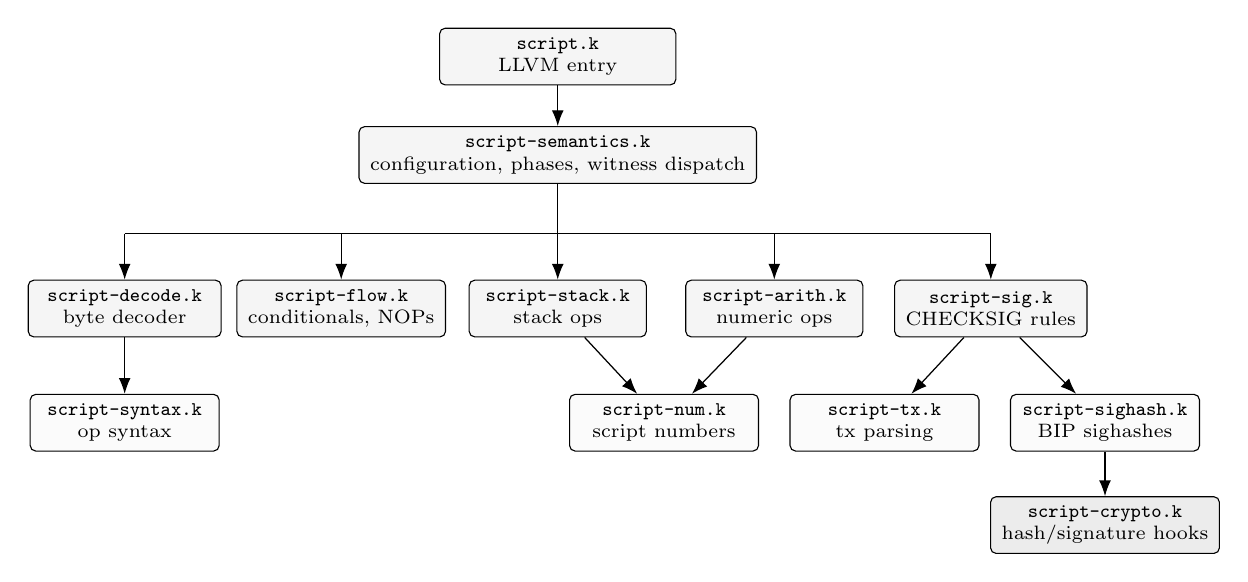
\begin{tikzpicture}[
    x=1cm,y=1cm,
    module/.style={draw, rounded corners=2pt, align=center, font=\scriptsize,
      minimum height=0.72cm, inner xsep=4pt, inner ysep=3pt, fill=gray!8},
    support/.style={module, fill=gray!3},
    hook/.style={module, fill=gray!15},
    edge/.style={-{Latex[length=2mm]}, line width=0.45pt},
    bus/.style={line width=0.45pt}
  ]
    \node[module, minimum width=3.0cm] (entry) at (0,4.6)
      {\texttt{script.k}\\LLVM entry};
    \node[module, minimum width=4.5cm] (core) at (0,3.35)
      {\texttt{script-semantics.k}\\configuration, phases, witness dispatch};

    \node[module, minimum width=2.45cm] (decode) at (-5.5,1.4)
      {\texttt{script-decode.k}\\byte decoder};
    \node[module, minimum width=2.35cm] (flow) at (-2.75,1.4)
      {\texttt{script-flow.k}\\conditionals, NOPs};
    \node[module, minimum width=2.25cm] (stack) at (0,1.4)
      {\texttt{script-stack.k}\\stack ops};
    \node[module, minimum width=2.25cm] (arith) at (2.75,1.4)
      {\texttt{script-arith.k}\\numeric ops};
    \node[module, minimum width=2.35cm] (sig) at (5.5,1.4)
      {\texttt{script-sig.k}\\CHECKSIG rules};

    \node[support, minimum width=2.4cm] (syntax) at (-5.5,-0.05)
      {\texttt{script-syntax.k}\\op syntax};
    \node[support, minimum width=2.4cm] (num) at (1.35,-0.05)
      {\texttt{script-num.k}\\script numbers};
    \node[support, minimum width=2.4cm] (tx) at (4.15,-0.05)
      {\texttt{script-tx.k}\\tx parsing};
    \node[support, minimum width=2.4cm] (sighash) at (6.95,-0.05)
      {\texttt{script-sighash.k}\\BIP sighashes};
    \node[hook, minimum width=2.45cm] (crypto) at (6.95,-1.35)
      {\texttt{script-crypto.k}\\hash/signature hooks};

    \draw[edge] (entry) -- (core);
    \draw[bus] (core.south) -- (0,2.35);
    \draw[bus] (-5.5,2.35) -- (5.5,2.35);
    \draw[edge] (-5.5,2.35) -- (decode.north);
    \draw[edge] (-2.75,2.35) -- (flow.north);
    \draw[edge] (0,2.35) -- (stack.north);
    \draw[edge] (2.75,2.35) -- (arith.north);
    \draw[edge] (5.5,2.35) -- (sig.north);

    \draw[edge] (decode) -- (syntax);
    \draw[edge] (stack) -- (num);
    \draw[edge] (arith) -- (num);
    \draw[edge] (sig) -- (tx);
    \draw[edge] (sig) -- (sighash);
    \draw[edge] (sighash) -- (crypto);
  \end{tikzpicture}%
  }
  \caption{High-level organization of the executable K definition.  The core
  configuration and phase machinery live in \texttt{script-semantics.k}; most
  opcode families are separated into smaller modules, while cryptographic
  primitives are delegated to native hooks.}
  \label{fig:module-map}
\end{figure*}

Table~\ref{tab:modules} summarizes the role of each major module.  This split
is useful for audit.  A reader investigating stack behavior can stay mostly in
\texttt{script-stack.k}; a reader investigating BIP-341 serialization can go to
\texttt{script-sighash.k}; and a reader investigating phase boundaries can
start in \texttt{script-semantics.k}.  Some foundational push, stack, and hash
rules remain in the core module because they are shared by common templates and
the phase machinery.  Another exception is
\texttt{OP\_CODESEPARATOR}, whose behavior necessarily crosses modules: the
decoder records the byte tail after the separator, the flow and signature rules
respect whether the opcode was actually executed, and the sighash module
consumes the resulting script-code state.

\begin{table*}[t]
  \caption{Major K modules and their semantic responsibilities}
  \label{tab:modules}
  \centering
  \footnotesize
  \begin{tabular}{p{0.22\textwidth}p{0.28\textwidth}p{0.42\textwidth}}
    \toprule
    Module & Primary content & Why it is separated \\
    \midrule
    \texttt{script-semantics.k} &
    Configuration, phase sort, failure mechanism, witness dispatch, Taproot
    skeleton, cleanup rules &
    Owns global state and validation sequencing; most other modules import the
    declarations introduced here. \\
    \texttt{script-decode.k} &
    Byte-to-opcode dispatch, push-data decoding, opcode-count accounting,
    Tapscript \texttt{OP\_SUCCESSx} cases &
    Bitcoin Script is serialized bytecode; consensus behavior depends on how
    bytes are decoded, not just on the abstract opcode names. \\
    \texttt{script-flow.k} &
    \texttt{OP\_IF}, \texttt{OP\_NOTIF}, \texttt{OP\_ELSE},
    \texttt{OP\_ENDIF}, execution guarding, CLTV/CSV NOP behavior &
    Conditional execution determines whether most opcode rules fire or are
    skipped; centralizing the guard avoids duplicating branch logic. \\
    \texttt{script-stack.k}, \texttt{script-arith.k} &
    Local stack and numeric opcode rules &
    These rules are mostly phase-independent and mention only the stack,
    altstack, or script-number helpers. \\
    \texttt{script-sig.k} &
    ECDSA and Schnorr signature opcode rules, multisig collection,
    \texttt{OP\_CHECKSIGADD} &
    Signature opcodes are where stack state, consensus flags, transaction
    context, and phase-specific sighash construction meet. \\
    \texttt{script-sighash.k}, \texttt{script-tx.k} &
    Transaction field extraction, legacy/BIP-143/BIP-341/BIP-342 preimage
    construction &
    Sighash construction is byte-precise and large enough to deserve its own
    testable layer. \\
    \texttt{script-crypto.k} &
    Hash and signature hook boundaries &
    Primitive cryptography is delegated to native code, while selection and
    serialization remain in K. \\
    \bottomrule
  \end{tabular}
\end{table*}

\subsection{Configuration}

The top-level configuration is a single \kcell{T} cell containing the active
computation, stacks, validation phase, error state, input scripts, witness
blob, consensus flags, transaction context, and phase-specific signature
metadata.  Figure~\ref{fig:configuration} groups the most important cells by
role.  The actual K configuration is slightly more detailed, but the grouping
captures the design: ordinary opcodes see a small local state, while signature
and phase rules can mention the extra cells needed for consensus validation.

\begin{figure}[t]
  \centering
  \resizebox{\columnwidth}{!}{%
  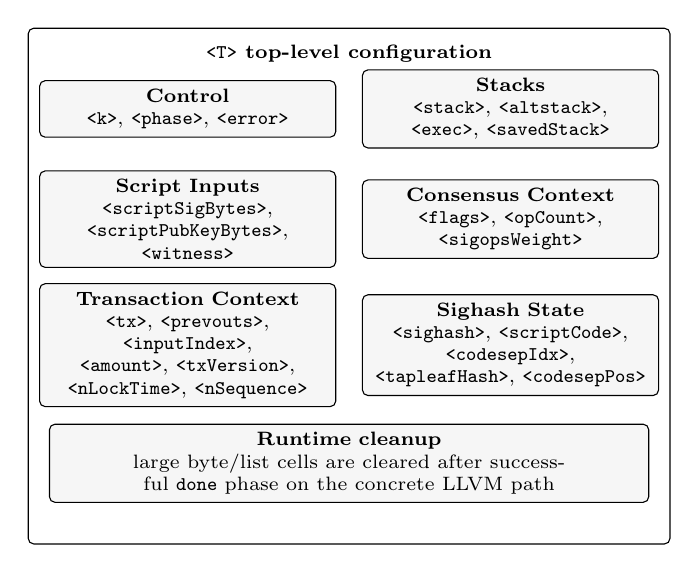
\begin{tikzpicture}[
    x=1cm,y=1cm,
    cell/.style={draw, rounded corners=2pt, align=center, font=\scriptsize,
      inner sep=3pt, fill=gray!7},
    group/.style={draw, rounded corners=2pt, align=center, font=\scriptsize,
      inner sep=4pt, fill=white}
  ]
    \node[group, minimum width=8.15cm, minimum height=6.55cm] (top) at (0,0) {};
    \node[font=\scriptsize\bfseries, anchor=north] at (0,3.18) {\kcell{T} top-level configuration};
    \node[cell, text width=3.55cm] at (-2.05,2.25)
      {\textbf{Control}\\\kcell{k}, \kcell{phase}, \kcell{error}};
    \node[cell, text width=3.55cm] at (2.05,2.25)
      {\textbf{Stacks}\\\kcell{stack}, \kcell{altstack}, \kcell{exec}, \kcell{savedStack}};
    \node[cell, text width=3.55cm] at (-2.05,0.85)
      {\textbf{Script Inputs}\\\kcell{scriptSigBytes}, \kcell{scriptPubKeyBytes}, \kcell{witness}};
    \node[cell, text width=3.55cm] at (2.05,0.85)
      {\textbf{Consensus Context}\\\kcell{flags}, \kcell{opCount}, \kcell{sigopsWeight}};
    \node[cell, text width=3.55cm] at (-2.05,-0.75)
      {\textbf{Transaction Context}\\\kcell{tx}, \kcell{prevouts}, \kcell{inputIndex}, \kcell{amount},
      \kcell{txVersion}, \kcell{nLockTime}, \kcell{nSequence}};
    \node[cell, text width=3.55cm] at (2.05,-0.75)
      {\textbf{Sighash State}\\\kcell{sighash}, \kcell{scriptCode}, \kcell{codesepIdx},
      \kcell{tapleafHash}, \kcell{codesepPos}};
    \node[cell, text width=7.4cm] at (0,-2.25)
      {\textbf{Runtime cleanup}\\large byte/list cells are cleared after successful \texttt{done} phase
      on the concrete LLVM path};
  \end{tikzpicture}%
  }
  \caption{Simplified view of the K configuration.  Rewrite rules mention only
  the cells they need, which keeps ordinary opcode rules local while still
  allowing signature and phase rules to inspect transaction context.}
  \label{fig:configuration}
\end{figure}

The \kcell{k} cell starts at \texttt{\#init}.  Initialization checks
\texttt{scriptSig} size and push-only requirements, then schedules decoding of
either the unlocking script or the locking script.  The data stack is
\kcell{stack}; \kcell{altstack} models the Script altstack; and \kcell{exec}
stores a list of booleans representing nested conditional-execution state.
Most stack, arithmetic, and hash opcodes rewrite only \kcell{k} and
\kcell{stack}.  For example, a simple stack operation does not need to know
the spending transaction, the previous output set, or the witness.

The phase and consensus cells make the same opcode name meaningful in the
right validation regime.  \kcell{phase} ranges over
\texttt{scriptSig}, \texttt{scriptPubKey}, \texttt{p2sh-redeem},
\texttt{witness-v0}, \texttt{witness-v1}, and \texttt{done}.  The
\kcell{flags} bitmask models Bitcoin Core verification flags such as
\texttt{FLAG\_P2SH}, \texttt{FLAG\_WITNESS}, \texttt{FLAG\_MINIMALDATA}, and
\texttt{FLAG\_TAPROOT}.  Rules can therefore express statements such as:
``in witness phases, if \texttt{MINIMALIF} is active, \texttt{OP\_IF} may only
consume an empty vector or \texttt{0x01}.''  This avoids baking one global
interpretation of an opcode into the syntax.

The transaction context is explicit rather than hidden in a host callback.
\kcell{tx} stores the serialized spending transaction, \kcell{prevouts}
stores the previous outputs needed by SegWit and Taproot hashing,
\kcell{inputIndex} selects the input under validation, and \kcell{amount}
carries the spent-output amount.  Older fixtures can still supply a
precomputed \kcell{sighash} blob, but the main benchmark path uses K-side
sighash construction from \kcell{tx} and \kcell{prevouts}.  This is the
difference between merely replaying Bitcoin Core's answer and specifying how
the answer is obtained.

Several cells exist specifically for script-code tracking.  Legacy, BIP-143,
and BIP-342 all depend on the portion of the script committed to by a
signature, but they do so differently.  For SegWit v0, \kcell{scriptCode}
stores the current BIP-143 script code.  For legacy signatures, it is an
override populated after an executed \texttt{OP\_CODESEPARATOR}; otherwise the
legacy sighash rules derive the script code from the active
\texttt{scriptSig}, \texttt{scriptPubKey}, or P2SH redeem bytes.  The
\kcell{pendingCodesepTail} cell is written by the decoder just before a decoded
\texttt{OP\_CODESEPARATOR}; if the separator is actually executed, the opcode
rule can promote that tail into \kcell{scriptCode}.  Tapscript uses
\kcell{tapleafHash}, \kcell{tapscriptBytes}, and \kcell{codesepPos} for the
BIP-342 extension fields.

\begin{table}[t]
  \caption{Selected configuration cells}
  \label{tab:cells}
  \centering
  \footnotesize
  \resizebox{\columnwidth}{!}{%
  \begin{tabular}{lll}
    \toprule
    Cell & Kind of state & Read by \\
    \midrule
    \kcell{k} & Pending computation & All rules \\
    \kcell{stack}, \kcell{altstack} & Script data stacks & Opcode rules \\
    \kcell{exec} & Conditional branch stack & Flow guard, IF/ELSE/ENDIF \\
    \kcell{phase} & Current validation phase & Phase, signature, decoder rules \\
    \kcell{flags} & Consensus verification flags & Phase and opcode guards \\
    \kcell{tx}, \kcell{prevouts} & Serialized tx context & Sighash rules \\
    \kcell{witness} & Witness stack blob & Witness and Taproot dispatch \\
    \kcell{scriptCode} & BIP-143 code or legacy CODESEPARATOR override & Signature rules \\
    \kcell{tapleafHash} & Tapscript leaf commitment & BIP-342 sighash \\
    \kcell{error} & Bitcoin Core-style error code & Harness and tests \\
    \bottomrule
  \end{tabular}
  }
\end{table}

The configuration also includes a concrete-runtime cleanup rule.  Once an
ordinary successful path reaches \texttt{done} and the \kcell{k} cell drains,
the LLVM backend rewrites large byte and list cells such as \kcell{tx},
\kcell{prevouts}, \kcell{witness}, and \kcell{sighash} to empty values.  This
rule is tagged concrete so proof-oriented backends do not see it.  Taproot
key-path success is currently a special terminal path: the successful
\texttt{\#taprootVerify} rule drains \kcell{k} directly rather than transitioning
through \texttt{done}, so it does not use this cleanup rule.  The rule does not
change the result observed by the verifier, which reads only success/failure and
the final error state, but it dramatically reduces the final KORE pattern that
the runtime must serialize for the paths that do reach \texttt{done}.

\subsection{Execution Phases}

Script validation is modeled as a phase machine rather than as one monolithic
interpreter loop.  Figure~\ref{fig:phase-flow} gives the high-level flow.
Every ordinary script phase has the same inner shape: decode a byte string,
execute the scheduled opcode computations, and then run \texttt{\#phaseComplete}
to decide the next phase.  That decision depends on the stack, flags, script
templates, witness data, and phase-specific validity checks.

\begin{figure*}[t]
  \centering
  \resizebox{\textwidth}{!}{%
  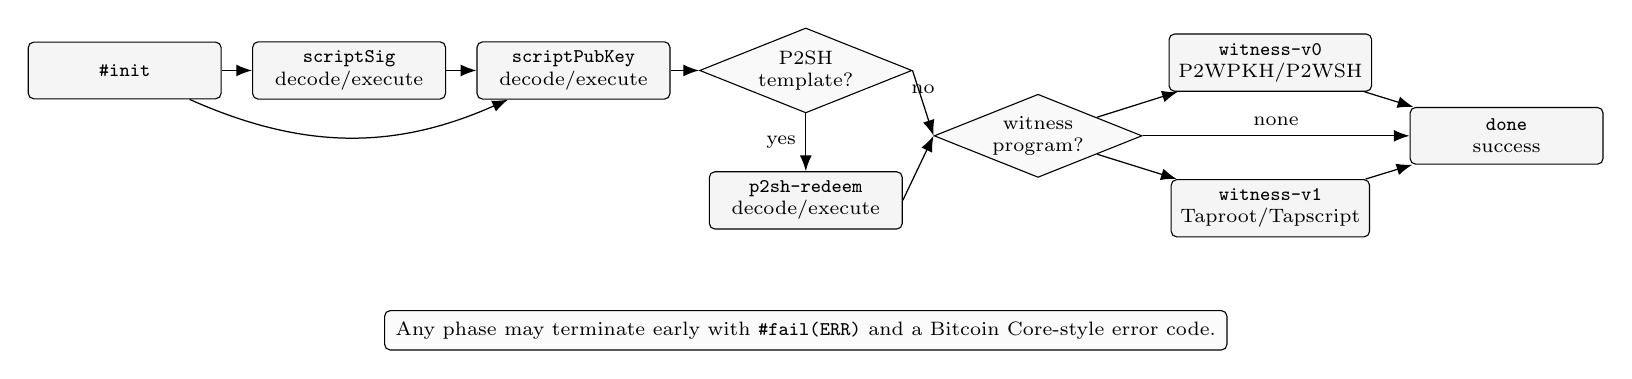
\begin{tikzpicture}[
    x=1cm,y=1cm,
    state/.style={draw, rounded corners=2pt, align=center, font=\scriptsize,
      minimum width=2.45cm, minimum height=0.72cm, fill=gray!8},
    decision/.style={draw, diamond, aspect=2.5, align=center, font=\scriptsize,
      inner sep=1pt, fill=gray!5},
    note/.style={draw, rounded corners=2pt, align=center, font=\scriptsize,
      inner sep=4pt, fill=gray!3},
    edge/.style={-{Latex[length=2mm]}, line width=0.45pt}
  ]
    \node[state] (init) at (0,2.25) {\texttt{\#init}};
    \node[state] (sig) at (2.85,2.25) {\texttt{scriptSig}\\decode/execute};
    \node[state] (pk) at (5.7,2.25) {\texttt{scriptPubKey}\\decode/execute};
    \node[decision] (p2sh) at (8.65,2.25) {P2SH\\template?};

    \node[state] (redeem) at (8.65,0.6) {\texttt{p2sh-redeem}\\decode/execute};
    \node[decision] (wit) at (11.6,1.42) {witness\\program?};
    \node[state] (wv0) at (14.55,2.35) {\texttt{witness-v0}\\P2WPKH/P2WSH};
    \node[state] (wv1) at (14.55,0.5) {\texttt{witness-v1}\\Taproot/Tapscript};
    \node[state] (done) at (17.55,1.42) {\texttt{done}\\success};
    \node[note, minimum width=8.5cm] (fail) at (8.65,-1.05)
      {Any phase may terminate early with \texttt{\#fail(ERR)} and a Bitcoin Core-style error code.};

    \draw[edge] (init) -- (sig);
    \draw[edge] (sig) -- (pk);
    \draw[edge] (init) to[bend right=24] (pk);
    \draw[edge] (pk) -- (p2sh);
    \draw[edge] (p2sh.south) -- node[left,font=\scriptsize] {yes} (redeem.north);
    \draw[edge] (p2sh.east) -- node[above,font=\scriptsize] {no} (wit.west);
    \draw[edge] (redeem.east) -- (wit.west);
    \draw[edge] (wit) -- (wv0);
    \draw[edge] (wit) -- (wv1);
    \draw[edge] (wit.east) -- node[above,font=\scriptsize] {none} (done.west);
    \draw[edge] (wv0) -- (done);
    \draw[edge] (wv1) -- (done);
  \end{tikzpicture}%
  }
  \caption{Simplified phase machine for script verification.  The curved
  \texttt{\#init}-to-\texttt{scriptPubKey} edge is the empty-\texttt{scriptSig}
  path; the witness branch targets either v0 or v1 script execution.  The
  Taproot key-path case is a terminal \texttt{\#taprootVerify} check rather than
  a \texttt{witness-v1} script phase.  The actual K rules include additional
  side conditions such as push-only checks,
  \texttt{WITNESS\_MALLEATED}, \texttt{WITNESS\_UNEXPECTED}, clean-stack checks,
  witness-program length checks, and Taproot control-block validation.}
  \label{fig:phase-flow}
\end{figure*}

The initial phase is \texttt{scriptSig}.  If the unlocking script is empty,
the semantics skips directly to \texttt{scriptPubKey}; otherwise it checks the
10,000-byte script-size limit and, when the flag is active, verifies that the
unlocking script is push-only.  After \texttt{scriptSig} completes, the rules
clear the altstack, reset the opcode count, reset code-separator state, and
schedule the locking script.

The \texttt{scriptPubKey} completion rules are the first major branch point.
If the locking script is a P2SH template under \texttt{FLAG\_P2SH}, the
semantics restores the saved stack from \texttt{scriptSig}, extracts the
redeem script, and enters \texttt{p2sh-redeem}.  If it is a native witness
program under \texttt{FLAG\_WITNESS}, it dispatches to
\texttt{\#witnessVerify}.  Otherwise the phase can finish directly, subject to
clean-stack and unexpected-witness checks in K; the final top-stack success
predicate is currently performed by Python after it inspects the terminated K
configuration.

The \texttt{p2sh-redeem} phase mirrors the post-\texttt{scriptPubKey}
decision, but with the redeem script as the candidate witness program.  This
is how P2SH-wrapped SegWit spends are modeled.  A redeem script that is not a
witness program finishes through the ordinary clean-stack path; a redeem
script that is a witness program enters the witness verifier.  As with direct
\texttt{scriptPubKey} completion, final success for this ordinary non-witness
path is observed by the wrapper after K terminates.  This split is
one reason the phase cell is useful: P2SH redeem execution, native witness
execution, and Tapscript execution all run decoded opcodes, but their boundary
conditions differ.

Witness version 0 is split by program length.  A 20-byte program is P2WPKH:
the witness must contain exactly a signature and public key, and the semantics
synthesizes the standard P2PKH script template before execution.  A 32-byte
program is P2WSH: the last witness item is the witness script, its SHA-256 hash
must equal the program, and all preceding witness items become the initial
stack.  In both cases the phase becomes \texttt{witness-v0}, the witness is
marked consumed, and \texttt{\#witnessComplete} enforces exactly one truthy
final stack item.

Witness version 1 dispatches to Taproot when \texttt{FLAG\_TAPROOT} is set and
the witness program is 32 bytes.  A single effective witness item is a key-path
spend: the semantics checks Schnorr signature shape, computes the BIP-341
sighash, and verifies the signature against the output key.  More than one
effective witness item is a script-path spend: the semantics validates the
control block, computes the TapLeaf commitment, pushes the script-path witness
items, decodes the tapscript, and enters \texttt{witness-v1}.  Tapscript then
finishes through \texttt{\#tapscriptComplete}, again requiring one truthy item
on the final stack.

\begin{table}[t]
  \caption{Validation phases}
  \label{tab:phases}
  \centering
  \footnotesize
  \resizebox{\columnwidth}{!}{%
  \begin{tabular}{lll}
    \toprule
    Phase & Input executed & Main exit decision \\
    \midrule
    \texttt{scriptSig} & Unlocking script & Schedule \texttt{scriptPubKey} \\
    \texttt{scriptPubKey} & Locking script & Finish, P2SH, or witness dispatch \\
    \texttt{p2sh-redeem} & Redeem script & Finish or witness dispatch \\
    \texttt{witness-v0} & P2WPKH/P2WSH script & BIP-143 clean-stack completion \\
    \texttt{witness-v1} & Tapscript & BIP-342 completion and budget rules \\
    \texttt{done} & None & Ordinary success cleanup \\
    \bottomrule
  \end{tabular}
  }
\end{table}

Many failures are explicit.  The K item \texttt{\#fail(ERR)} writes a Bitcoin
Core-style error string into \kcell{error} and clears \kcell{k}.  Negative test
vectors for covered error paths therefore terminate with structured failure
labels such as \texttt{SCRIPT\_SIZE}, \texttt{SIG\_PUSHONLY},
\texttt{WITNESS\_PROGRAM\_MISMATCH}, \texttt{CLEANSTACK}, or
\texttt{SCHNORR\_SIG}.  Some ill-formed states, such as stack underflow in a
rule whose left-hand side cannot match, are still represented as stuck K terms;
the Python harness treats those as implicit failures.  This is valuable for
debugging because a mismatch can be classified as the wrong success value, the
wrong error class, a stuck execution, or a harness problem before looking at the
full configuration trace.

\subsection{Decoder and Guarded Execution}

The decoder is the part of the definition that most directly reflects Bitcoin
Script's bytecode nature.  It consumes a \texttt{Bytes} value, inspects the
first byte, schedules the corresponding opcode computation, and recursively
continues on the tail.  Figure~\ref{fig:decoder} shows the pipeline.  The
decoder has to do more than map bytes to names: it enforces script-element
size, counts opcodes above \texttt{OP\_16}, identifies disabled and reserved
opcodes, handles \texttt{OP\_SUCCESSx} in Tapscript, and records byte tails for
\texttt{OP\_CODESEPARATOR}.

\begin{figure*}[t]
  \centering
  \resizebox{0.96\textwidth}{!}{%
  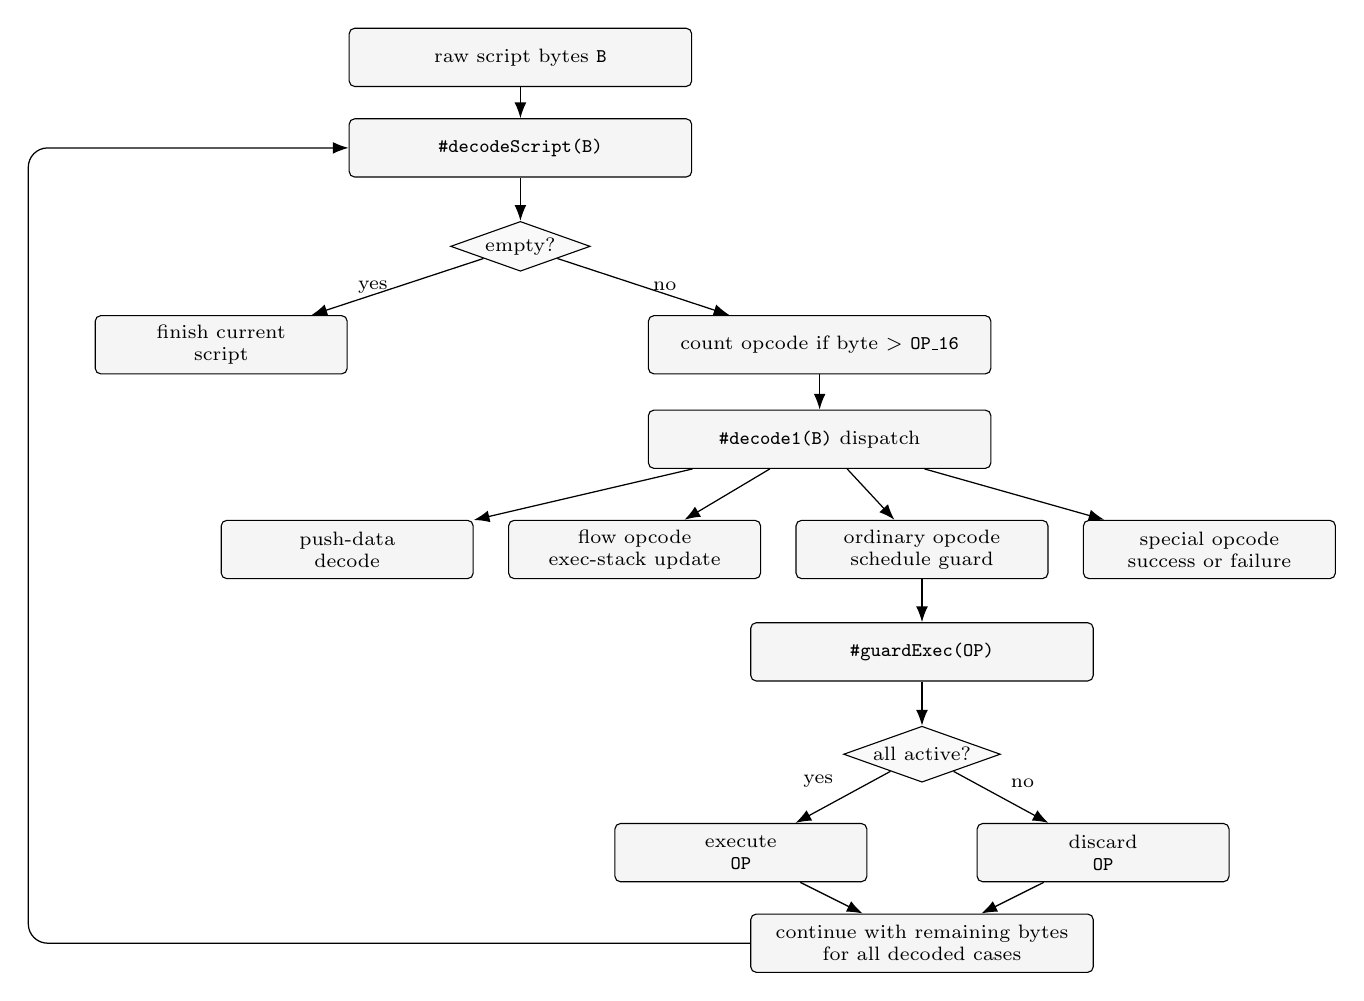
\begin{tikzpicture}[
    x=1cm,y=1cm,
    dstep/.style={draw, rounded corners=2pt, align=center, font=\scriptsize,
      minimum width=3.2cm, minimum height=0.74cm, inner xsep=4pt, fill=gray!8},
    wide/.style={dstep, minimum width=4.35cm},
    branch/.style={draw, diamond, aspect=2.8, align=center, font=\scriptsize,
      inner sep=1pt, fill=gray!5},
    edge/.style={-{Latex[length=2mm]}, line width=0.45pt},
    back/.style={-{Latex[length=2mm]}, line width=0.45pt, rounded corners=7pt}
  ]
    \node[wide] (bytes) at (0,5.2) {raw script bytes \texttt{B}};
    \node[wide] (decode) at (0,4.05) {\texttt{\#decodeScript(B)}};
    \node[branch] (empty) at (0,2.8) {empty?};
    \node[dstep] (finish) at (-3.8,1.55) {finish current\\script};
    \node[wide] (count) at (3.8,1.55) {count opcode if byte $>$ \texttt{OP\_16}};
    \node[wide] (decodeone) at (3.8,0.35) {\texttt{\#decode1(B)} dispatch};

    \node[dstep] (push) at (-2.2,-1.05) {push-data\\decode};
    \node[dstep] (flow) at (1.45,-1.05) {flow opcode\\exec-stack update};
    \node[dstep] (ordinary) at (5.1,-1.05) {ordinary opcode\\schedule guard};
    \node[dstep] (special) at (8.75,-1.05) {special opcode\\success or failure};

    \node[wide] (guard) at (5.1,-2.35) {\texttt{\#guardExec(OP)}};
    \node[branch] (active) at (5.1,-3.65) {all active?};
    \node[dstep] (execute) at (2.8,-4.9) {execute\\\texttt{OP}};
    \node[dstep] (discard) at (7.4,-4.9) {discard\\\texttt{OP}};
    \node[wide] (tail) at (5.1,-6.05) {continue with remaining bytes\\for all decoded cases};

    \draw[edge] (bytes) -- (decode);
    \draw[edge] (decode) -- (empty);
    \draw[edge] (empty) -- node[left,font=\scriptsize] {yes} (finish);
    \draw[edge] (empty) -- node[right,font=\scriptsize] {no} (count);
    \draw[edge] (count) -- (decodeone);
    \draw[edge] (decodeone) -- (push);
    \draw[edge] (decodeone) -- (flow);
    \draw[edge] (decodeone) -- (ordinary);
    \draw[edge] (decodeone) -- (special);
    \draw[edge] (ordinary) -- (guard);
    \draw[edge] (guard) -- (active);
    \draw[edge] (active) -- node[above left,font=\scriptsize] {yes} (execute);
    \draw[edge] (active) -- node[above right,font=\scriptsize] {no} (discard);
    \draw[edge] (execute) -- (tail);
    \draw[edge] (discard) -- (tail);
    \draw[back] (tail.west) -- (-6.25,-6.05) -- (-6.25,4.05) -- (decode.west);
  \end{tikzpicture}%
  }
  \caption{Decoder pipeline.  The decoder schedules executable K items while
  preserving byte-level resource checks and phase-sensitive special cases.}
  \label{fig:decoder}
\end{figure*}

The central scheduling idiom is:
\[
  \texttt{\#guardExec(OP)} \sim> \texttt{\#decodeScript(rest)}.
\]
The first component executes the opcode if the current conditional-execution
stack is active; the second component continues decoding the remaining byte
string.  Flow-control opcodes such as \texttt{OP\_IF}, \texttt{OP\_ELSE}, and
\texttt{OP\_ENDIF} are emitted directly because they must update
\kcell{exec} even in contexts where ordinary opcodes are skipped.  This matches
Bitcoin Script's rule that disabled branches still have to be structurally
balanced.

\texttt{\#guardExec} is defined in \texttt{script-flow.k}.  If every entry in
\kcell{exec} is true, the guard rewrites to the opcode and the opcode rule
fires.  If any entry is false, the guard rewrites to \texttt{.K}, dropping the
opcode without touching the stack.  This small abstraction is one of the
cleaner parts of the definition: it keeps skipped-branch behavior out of the
hundreds of ordinary opcode rules.  A stack opcode such as \texttt{OP\_DUP}
can be written as a local stack rewrite; the guard is responsible for deciding
whether that local rewrite is even reached.

Push-data decoding is also semantic.  \texttt{OP\_PUSHBYTES\_1} through
\texttt{OP\_PUSHBYTES\_75}, \texttt{OP\_PUSHDATA1},
\texttt{OP\_PUSHDATA2}, and \texttt{OP\_PUSHDATA4} all compute a length,
extract that many bytes, enforce the 520-byte push-size limit, and emit
\texttt{OP\_PUSHDATA(opcode,data)}.  Minimal-push checks are intentionally
performed at execution time instead of pure decode time, because
\texttt{MINIMALDATA} should not reject a non-minimal push inside a branch that
is not executed.  This is a good example of where an executable semantics has
to follow the consensus interpreter's control-flow sensitivity rather than a
cleaner context-free parser design.

The decoder is also phase-sensitive in Tapscript.  Several byte values that
are invalid or reserved in earlier phases become \texttt{OP\_SUCCESSx} in
\texttt{witness-v1}.  The K rule for such a byte checks \kcell{phase}; in
Tapscript it schedules \texttt{\#opSuccess}, which clears the remaining
computation and leaves a truthy value on the stack.  Outside Tapscript, the
same byte may become a reserved-opcode failure or an invalid-opcode failure.
This is another reason phase is explicit state rather than a parameter hidden
in the harness.

\begin{table}[t]
  \caption{Decoder responsibilities}
  \label{tab:decoder}
  \centering
  \footnotesize
  \resizebox{\columnwidth}{!}{%
  \begin{tabular}{ll}
    \toprule
    Responsibility & K mechanism \\
    \midrule
    Script byte iteration & \texttt{\#decodeScript} and \texttt{\#decode1} \\
    Opcode resource limit & \texttt{\#countOp}, \texttt{\#countOps} \\
    Push extraction & \texttt{\#decodePush(opcode, length, rest)} \\
    Conditional skipping & \texttt{\#guardExec(OP)} over \kcell{exec} \\
    Minimal-push timing & Execution-time \texttt{\#isMinimalPush} checks \\
    Code separator tracking & \texttt{\#setCodesepTail} before opcode execution \\
    Tapscript success opcodes & Phase-sensitive \texttt{\#opSuccess} rules \\
    \bottomrule
  \end{tabular}
  }
\end{table}

\subsection{Opcode Families}

After decoding, most opcodes fall into small rule families.  Stack opcodes
rewrite \kcell{stack} and occasionally \kcell{altstack}.  Arithmetic opcodes
convert byte vectors into Bitcoin Script numbers, enforce numeric-size limits,
perform an integer operation, and push the minimally encoded result.  Hash
opcodes pop one byte vector, call a hash hook, and push the resulting digest.
Locktime and sequence opcodes consult \kcell{nLockTime}, \kcell{nSequence},
and verification flags.

Signature opcodes are the exception to the local-rule pattern.  Legacy
\texttt{OP\_CHECKSIG} must know the public key, signature, hash type, active
script code, and transaction serialization.  \texttt{OP\_CHECKMULTISIG} has
to collect variable-length public-key and signature lists, handle the
historical dummy element, count signature operations, and apply
\texttt{NULLDUMMY}/\texttt{NULLFAIL}.  Tapscript adds
\texttt{OP\_CHECKSIGADD}, Schnorr signature-shape checks, public-key-type
rules, and a signature validation budget.  For this reason the signature
module is where many cells meet: \kcell{stack}, \kcell{phase}, \kcell{flags},
\kcell{scriptCode}, \kcell{tx}, \kcell{prevouts}, \kcell{inputIndex},
\kcell{amount}, \kcell{tapleafHash}, and \kcell{sigopsWeight}.

This organization keeps the readable part of the semantics close to the
language structure.  A reader can treat ordinary opcodes as small rewrite
rules and signature opcodes as phase-dispatching rules.  The latter select
between legacy, BIP-143, BIP-341, and BIP-342 sighash helpers, then call the
appropriate ECDSA or Schnorr hook.  The hook boundary is deliberately narrow:
the hook verifies a cryptographic predicate over bytes, while K constructs the
bytes and chooses the predicate.

\subsection{Signature Hashing}

Signature checking is the largest semantic surface in the project.  Legacy
ECDSA checks use the legacy preimage rules, with support for historical
hash-type behavior.  SegWit v0 checks route through BIP-143.  Taproot key-path
and Tapscript checks route through BIP-341 and BIP-342.  Native hooks implement
primitive cryptographic operations and bulk SHA-256 walkers, while the K rules
own the selection logic, serialization layout, and phase-dependent dispatch.

This boundary follows the precedent of prior K definitions: primitive
operations may be hooked for execution, but semantic structure stays in K.  The
result is a definition that can run mainnet-sized transactions without asking K
to perform every byte-level hashing loop one byte at a time.  It also makes
the validation story more meaningful.  When K and Core agree on a Taproot
input, the agreement covers the witness layout, annex handling, control-block
validation, TapLeaf hash, sighash serialization, and Schnorr predicate, not
just an externally supplied digest.

\begin{figure*}[t]
  \centering
  \resizebox{\textwidth}{!}{%
  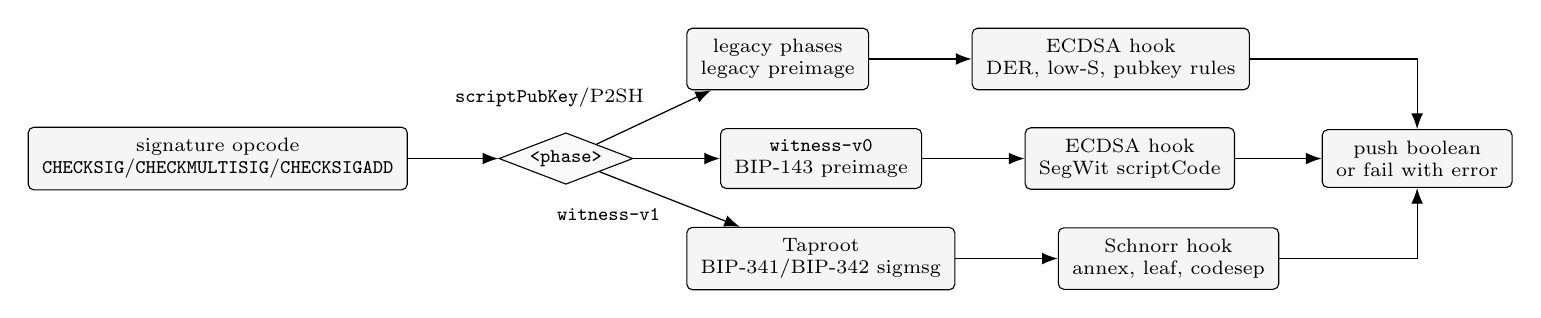
\begin{tikzpicture}[
    node distance=0.75cm and 0.9cm,
    block/.style={draw, rounded corners=2pt, align=center, font=\scriptsize,
      minimum height=0.72cm, inner xsep=5pt, inner ysep=4pt, fill=gray!8},
    choice/.style={draw, diamond, aspect=2.6, align=center, font=\scriptsize,
      inner sep=1pt, fill=gray!5},
    edge/.style={-{Latex[length=2mm]}, line width=0.45pt}
  ]
    \node[block, minimum width=2.9cm] (op)
      {signature opcode\\\texttt{CHECKSIG}/\texttt{CHECKMULTISIG}/\texttt{CHECKSIGADD}};
    \node[choice, right=1.15cm of op] (phase) {\kcell{phase}};
    \node[block, above right=0.7cm and 1.1cm of phase] (legacy)
      {legacy phases\\legacy preimage};
    \node[block, right=1.1cm of phase] (b143)
      {\texttt{witness-v0}\\BIP-143 preimage};
    \node[block, below right=0.7cm and 1.1cm of phase] (tap)
      {Taproot\\BIP-341/BIP-342 sigmsg};
    \node[block, right=1.3cm of legacy] (ecdsa)
      {ECDSA hook\\DER, low-S, pubkey rules};
    \node[block, right=1.3cm of b143] (ecdsa2)
      {ECDSA hook\\SegWit scriptCode};
    \node[block, right=1.3cm of tap] (schnorr)
      {Schnorr hook\\annex, leaf, codesep};
    \node[block, right=1.1cm of ecdsa2] (result)
      {push boolean\\or fail with error};

    \draw[edge] (op) -- (phase);
    \draw[edge] (phase) -- node[above left,font=\scriptsize] {\texttt{scriptPubKey}/P2SH} (legacy);
    \draw[edge] (phase) -- (b143);
    \draw[edge] (phase) -- node[below left,font=\scriptsize] {\texttt{witness-v1}} (tap);
    \draw[edge] (legacy) -- (ecdsa);
    \draw[edge] (b143) -- (ecdsa2);
    \draw[edge] (tap) -- (schnorr);
    \draw[edge] (ecdsa) -| (result);
    \draw[edge] (ecdsa2) -- (result);
    \draw[edge] (schnorr) -| (result);
  \end{tikzpicture}%
  }
  \caption{Signature-hash dispatch.  The signature opcode rules select a
  preimage algorithm from the current phase and then call a narrow
  cryptographic hook over the bytes constructed by K.}
  \label{fig:sighash-dispatch}
\end{figure*}

Figure~\ref{fig:sighash-dispatch} shows the dispatch at a high level.  Legacy
and P2SH execution use ECDSA over the historical transaction digest.  SegWit
v0 uses ECDSA over BIP-143, with \kcell{scriptCode} set either to the
canonical P2WPKH template or to the current P2WSH witness script.  Taproot
key-path spends use BIP-341 directly.  Tapscript spends use BIP-342's
extension fields: the tapleaf hash, key version, and code-separator position
are part of the signed message.  The K definition keeps these choices in the
rewrite rules rather than in the wrapper, so a phase bug appears as a semantic
bug, not as an invisible host-language dispatch.

\subsection{Spend-Shape Walkthroughs}

The phase machine is easiest to read through common spend shapes.
Table~\ref{tab:spend-shapes} lists paths for representative cases.  These are
not additional algorithms beyond the K rules; they are useful mental traces
through the executable definition.

\begin{table*}[t]
  \caption{Common spend shapes as paths through the K semantics}
  \label{tab:spend-shapes}
  \centering
  \footnotesize
  \begin{tabular}{p{0.18\textwidth}p{0.31\textwidth}p{0.43\textwidth}}
    \toprule
    Spend shape & Phase path & Key semantic events \\
    \midrule
    Legacy P2PKH or bare script &
    \texttt{scriptSig} $\rightarrow$ \texttt{scriptPubKey} $\rightarrow$
    \texttt{done} &
    \texttt{scriptSig} pushes unlocking data; \texttt{scriptPubKey} consumes
    it; signature opcodes use the legacy preimage and ECDSA hook. \\
    P2SH &
    \texttt{scriptSig} $\rightarrow$ \texttt{scriptPubKey} $\rightarrow$
    \texttt{p2sh-redeem} $\rightarrow$ \texttt{done} &
    The stack after \texttt{scriptSig} is saved; the redeem script is popped
    from the saved stack and decoded only after the P2SH template succeeds. \\
    Native P2WPKH &
    \texttt{scriptPubKey} $\rightarrow$ \texttt{witness-v0} $\rightarrow$
    \texttt{done} &
    Empty \texttt{scriptSig}; witness must contain signature and pubkey;
    K synthesizes the standard P2PKH template and uses it as BIP-143
    \kcell{scriptCode}. \\
    Native P2WSH &
    \texttt{scriptPubKey} $\rightarrow$ \texttt{witness-v0} $\rightarrow$
    \texttt{done} &
    Last witness item is hashed and compared with the witness program; earlier
    witness items become the initial stack; the witness script becomes
    \kcell{scriptCode}. \\
    Taproot key path &
    \texttt{scriptPubKey} $\rightarrow$ \texttt{\#taprootVerify} &
    A single effective witness item is checked as a Schnorr signature over the
    BIP-341 message; on success the K computation drains without decoding
    tapscript or entering \texttt{done}. \\
    Taproot script path &
    \texttt{scriptPubKey} $\rightarrow$ \texttt{\#taprootVerify}
    $\rightarrow$ \texttt{witness-v1} $\rightarrow$ \texttt{done} &
    Control block validates the output key; K computes the TapLeaf hash,
    pushes script-path witness items, decodes the tapscript, and enforces
    BIP-342 completion rules. \\
    \bottomrule
  \end{tabular}
\end{table*}

Consider native P2WPKH as a compact example.  The initial \texttt{scriptSig}
is empty, so \texttt{\#init} schedules the locking script directly and sets the
phase to \texttt{scriptPubKey}.  The locking script decodes to a witness
program.  On phase completion, the rules check that the witness flag is active
and that the unlocking script was empty, then call
\texttt{\#witnessVerify(0,PROG)}.  Because \texttt{PROG} is 20 bytes, the
rules require exactly two witness items, push them onto \kcell{stack}, build
the canonical P2PKH byte string, store that byte string in \kcell{scriptCode},
and decode it under \texttt{witness-v0}.  The ordinary P2PKH opcodes then run
through the same stack and signature rules used elsewhere, but
\texttt{OP\_CHECKSIG} dispatches to BIP-143 because the phase is
\texttt{witness-v0}.  Finally, \texttt{\#witnessComplete} requires exactly one
truthy stack item.

P2WSH follows the same witness-v0 completion discipline but differs in how the
executing script is chosen.  The last witness item is a byte string, not a
template synthesized by the semantics.  K computes its SHA-256 hash and
requires equality with the 32-byte witness program.  The earlier witness items
become the stack, and the witness script becomes both the decoded program and
the initial BIP-143 \kcell{scriptCode}.  \texttt{OP\_CODESEPARATOR} can then
update \kcell{scriptCode} during execution, but only when the separator is in
an executed branch.

Taproot script path is the richest trace.  \texttt{\#taprootVerify} first
removes a possible annex from the effective witness count, validates the
control-block size, computes the merkle path, and checks that the tweaked key
matches the output key.  Only after those structural checks succeed does the
semantics enter \texttt{witness-v1}.  At that point the tapscript bytes,
tapleaf hash, and code-separator position cells have been initialized for
BIP-342.  Tapscript opcodes then execute under the decoder's phase-sensitive
rules, which is what makes \texttt{OP\_SUCCESSx} successful in this phase but
not in earlier phases.

\subsection{Runtime Interface}

The Python wrapper constructs initial configurations and invokes the compiled
LLVM backend.  The latest runtime path avoids serializing the whole initial
configuration through textual KORE.  Instead, the wrapper uses the K LLVM C API
to build tokens and injections directly and calls the binary runtime path from
\texttt{verify\_script}.  The benchmark runner also goes through
\texttt{verify\_script}, ensuring the measured path is the same optimized path
used by normal verification.

The runtime interface is intentionally thin, but it is not completely
semantics-free.  It translates host data into K cells, starts the semantics, and
then classifies the final K pattern.  Opcode execution, phase dispatch, witness
handling, and K-side sighash construction live in the K definition.  The wrapper
still performs two observable boundary checks: it treats a nonempty \kcell{k}
cell as stuck execution, and it checks the final top-stack success predicate on
ordinary terminated paths.  In the current wrapper this final predicate is a
nonempty-byte check, so moving the full Bitcoin truthiness rule into K is a
remaining cleanup item.  This keeps the benchmark artifact primarily a K
semantics, while also identifying a consensus-significant boundary that should
eventually move into K.

\section{Validation}

\subsection{AI-Assisted Methodology}

The implementation process was intentionally agentic but ground-truth driven.
Claude Code session history for this repository records the main implementation
sessions as \texttt{claude-opus-4-6} and \texttt{claude-opus-4-7}, with a small
number of \texttt{claude-sonnet-4-6} side turns.  The final report and late
branch/benchmark recovery work used OpenAI Codex (GPT-5).  The human role was
to choose the architecture, define the validation targets, review the resulting
rules and harnesses, and decide ambiguous design questions that the tests alone
could not settle.

The reason this workflow was viable is that \bitcoin Script has unusually good
external oracles.  The development loop was not ``ask a model to write a
semantics and trust it.''  Instead, tasks were phrased as verifiable repairs:
make a failing Bitcoin Core \texttt{script\_tests.json} vector pass, close a
\texttt{tx\_valid.json}/\texttt{tx\_invalid.json} discrepancy, match a BIP-341
wallet vector, or agree with \texttt{libbitcoinconsensus} on a mainnet-derived
input.  Every substantial semantic change was checked against these artifacts,
and later against larger mainnet and benchmark runs.  Model output was useful
for navigating K rules, plumbing Python wrappers, and proposing fixes, but the
acceptance criterion was always agreement with the official vectors or with
Bitcoin Core's consensus library on concrete inputs.

This makes the process closer to test-driven semantic development than to
free-form code generation.  A failing vector supplied the specification for a
small change; the full vector suite and mainnet replay guarded against
regression; and benchmark comparison caught performance regressions such as the
temporary loss of the v10 binary K runner path.  In this setting, the AI agent
acted as an implementation accelerator inside a deterministic verification
loop, while the ground truth remained Bitcoin's published tests, BIP reference
data, and Core behavior.

\subsection{Reference Tests}

Table~\ref{tab:coverage} summarizes the current validation story.  The
semantics passes all 1,222 Bitcoin Core \texttt{script\_tests.json} vectors.
It also passes 201 of 214 transaction vectors.  The remaining 13 are documented
expected failures: nine malformed \texttt{BADTX} cases that exercise
transaction-level checks rather than script validation, one
\texttt{CODESEPARATOR}/\texttt{CONST\_SCRIPTCODE} divergence, and three cases
whose invalidity depends on verification flags deliberately excluded by the
harness.

\begin{table}[htbp]
  \caption{Reference test coverage}
  \label{tab:coverage}
  \centering
  \footnotesize
  \resizebox{\columnwidth}{!}{%
  \begin{tabular}{lrrl}
    \toprule
    Suite & Cases & Passing & Notes \\
    \midrule
    \texttt{script\_tests.json} & 1,222 & 1,222 & Standard, SegWit, Taproot \\
    \texttt{tx\_valid.json} & 121 & 121 & Transaction validation \\
    \texttt{tx\_invalid.json} & 93 & 80 & 13 expected xfails \\
    Taproot coverage cases & 26 & 26 & Derived from Core feature categories \\
    \bottomrule
  \end{tabular}
  }
\end{table}

\subsection{Sighash Tests}

Sighash coverage is split across several evidence sources.  The Bitcoin Core
script and transaction vector harnesses still provide precomputed sighash blobs
for many legacy and SegWit-v0 cases, so those tests validate opcode behavior
and signature dispatch without independently validating every sighash entry
point.  The main benchmark path, by contrast, passes the spending transaction
and previous outputs so K constructs the legacy, BIP-143, BIP-341, and BIP-342
messages during verification.  The repository also includes an end-to-end
BIP-341 wallet-vector test that forces the K-side key-path sighash by supplying
no precomputed blob.  Standalone legacy/BIP-143 vector files, direct C-hook
isolation tests, and direct BIP-342 script-path vector tests should be added to
make the coverage argument cleaner.

\subsection{Mainnet Dataset}

The benchmark dataset contains 288,190 real mainnet inputs from 72 blocks,
spanning pre-P2SH through Taproot-era transactions.  K is run in 29 subprocess
chunks to bound the LLVM runtime arena size; each chunk drops five warmup
inputs, producing 288,045 K result rows.  Core is run as a separate Core30 pass
and drops five warmup inputs once, producing 288,185 Core rows.  The combined
report contains the 288,045 paired rows for which both K and Core results are
available.  All paired rows agree.

\section{Formal Verification}

Beyond execution and testing, the \kframework provides a Haskell Kore prover
for symbolic proof of reachability claims.  K-Bitcoin Script includes 72 K
claims across 19 specification files.  The Haskell Kore prover discharges 70 of
them; two concrete HTLC hash-path claims are checked through the LLVM-backed
execution path because the Haskell prover does not yet evaluate the required
SHA-256 hook.

\subsection{Proof Infrastructure}

Each claim is a K reachability statement of the form $\langle\,\textit{init}\,\rangle
\Rightarrow \langle\,\textit{final}\,\rangle$, where \textit{init} specifies
a concrete or symbolic initial configuration and \textit{final} specifies the
expected outcome.  Claims import \texttt{SCRIPT-VERIFICATION}, a wrapper that
initializes the semantics under given consensus flags and scripts.  For the 70
claims in the Haskell prover suite, Kore discharges reachability by symbolic
execution over the rewrite rules, with arithmetic side conditions delegated to
an SMT backend.  The two concrete HTLC hash-path claims use the same K rules but
are checked through the LLVM path so the SHA-256 hook can be evaluated.

A notable engineering challenge arose with the Kore prover: it cannot
automatically discharge integer commutativity ($a +_{\mathbb{Z}} b =
b +_{\mathbb{Z}} a$).  This required ensuring that the K rule variable
convention (which stack slot is named $A$ vs.\ $B$) matches the spec convention
exactly, so that unification of the success post-condition is trivial rather
than requiring a rewrite lemma.

\subsection{Historical Bug Proofs}

Four pairs of claims formalize the semantic effect of four historical soft-fork
fixes.  Each pair has a \emph{permissive} claim (the exploit succeeds without
the flag) and a \emph{restrictive} claim (the exploit is blocked with the flag
active).

\begin{itemize}
  \item \textbf{BIP~62 / MINIMALDATA.}  \texttt{0x0000} is a non-minimal
  encoding of zero.  Without the flag, the script \texttt{<0x0000> OP\_NOT}
  succeeds (NOT of zero is one).  With the flag, the push is rejected and
  execution terminates with error \texttt{MINIMALDATA}.

  \item \textbf{BIP~147 / NULLDUMMY.}  \texttt{OP\_CHECKMULTISIG} pops an
  extra dummy element due to a historical off-by-one.  Without the flag, any
  dummy value is accepted, enabling third-party transaction malleability.  With
  the flag, a non-empty dummy raises \texttt{NULLDUMMY}.

  \item \textbf{CLEANSTACK.}  The script \texttt{OP\_1 OP\_1} leaves two truthy
  items without the flag, providing a covert data channel.  With the flag, the
  semantics requires exactly one item at completion and raises
  \texttt{CLEANSTACK}.

  \item \textbf{DISCOURAGE\_UPGRADABLE\_NOPS.}  Without the flag,
  \texttt{OP\_NOP1}--\texttt{OP\_NOP10} are harmless.  With it, any reserved
  NOP raises \texttt{DISCOURAGE\_UPGRADABLE\_NOPS}, preventing scripts from
  pre-committing to NOP-behavior before a soft fork repurposes the opcode (as
  NOP2 and NOP3 were repurposed for CLTV and CSV).
\end{itemize}

The permissive direction of each pair confirms that the semantics faithfully
models pre-fix behavior; the restrictive direction confirms that the fix closes
the vulnerability.  Together they constitute a machine-checked audit of four
consensus rule changes.

\subsection{Arithmetic and Stack Correctness}

A second group of claims verifies opcode-level correctness: that numeric
opcodes produce the correct minimally-encoded result for concrete inputs, and
that inputs violating the 4-byte CScriptNum limit raise the appropriate error.
For example, the \texttt{OP\_ADD} claim verifies that the minimal encoding of
$a$, followed by the minimal encoding of $b$, followed by \texttt{OP\_ADD},
leaves the minimal encoding of $a+b$ on the stack.  The corresponding fail
claim verifies that an oversized operand sets the \texttt{UNKNOWN\_ERROR} error
field.  The 72 total claims span arithmetic, stack manipulation, flow-control
boundaries, cryptographic shape checks, HTLC behavior, and the historical bug
categories described above.

\section{Quantitative Evaluation}

\subsection{Methodology}

The final benchmark was run on the remote M4 Pro machine previously used for
the v8--v10 benchmark series.  The repository was synced to
\texttt{origin/main} after PR~\#11, commit \texttt{d11942b}.  The K LLVM definition was
rebuilt from that commit.  K was measured with one iteration per input using
the chunked subprocess driver.  Core was measured with
\texttt{libbitcoinconsensus} from Bitcoin Core 27.2, using 30 iterations per
input to match the prior v10 artifact.  For each input, the benchmark records
the median timed verifier call.  Therefore the totals below are aggregates of
per-input medians, not stopwatch wall-clock duration for the full driver
process.  This matters because the Core30 pass repeats each input 30 times, and
because both engines do some per-input buffer preparation outside the timed
region.  K's one-iteration measurements are correspondingly noisier than Core's
30-iteration medians, so p95 values should be read as single-run latency
summaries rather than variance estimates.

\subsection{Overall Results}

Table~\ref{tab:overall} gives the main result.  Summing the paired per-input
timed verifier medians gives 175.4 seconds for K and 84.2 seconds for Core, for
an aggregate timed-call ratio of 2.1$\times$.

\begin{table}[htbp]
  \caption{Fresh merged-main benchmark, paired rows}
  \label{tab:overall}
  \centering
  \footnotesize
  \resizebox{\columnwidth}{!}{%
  \begin{tabular}{lrrrr}
    \toprule
    Engine & Inputs & Aggregate total & Throughput & Median \\
    \midrule
    K Framework & 288,045 & 175.4 s & 1,642.3/s & 375.8 $\mu$s \\
    \texttt{libbitcoinconsensus} & 288,045 & 84.2 s & 3,419/s & 27.1 $\mu$s \\
    \bottomrule
  \end{tabular}
  }
\end{table}

The median K noop baseline is 234.1 $\mu$s, so the median net verification
cost is about 141.8 $\mu$s.  Core's median noop baseline is about 1.0 $\mu$s,
with a median net verification cost of about 26.1 $\mu$s.  These no-op values
come from the standalone 100-iteration baseline embedded in the combined
benchmark artifact, not from the chunk metadata emitted by the one-iteration K
driver.

\subsection{Results by Era}

Table~\ref{tab:era} shows median and 95th-percentile latency by consensus era.
DERSIG has a high Core median because the dataset includes large historical
stress transactions.  The K median remains under 400 $\mu$s across all eras,
while its DERSIG p95 records the residual cost of the stress cases.

\begin{table}[htbp]
  \caption{Latency by consensus era}
  \label{tab:era}
  \centering
  \footnotesize
  \resizebox{\columnwidth}{!}{%
  \begin{tabular}{lrrrr}
    \toprule
    Era & Inputs & K med & K p95 & Core med \\
    \midrule
    pre-P2SH & 286 & 350.4 $\mu$s & 387.3 $\mu$s & 15.5 $\mu$s \\
    P2SH & 8,840 & 353.8 $\mu$s & 484.5 $\mu$s & 17.3 $\mu$s \\
    DERSIG & 59,479 & 364.0 $\mu$s & 4.8 ms & 2.1 ms \\
    CLTV & 42,167 & 385.8 $\mu$s & 880.0 $\mu$s & 27.5 $\mu$s \\
    CSV & 39,361 & 379.6 $\mu$s & 834.1 $\mu$s & 23.4 $\mu$s \\
    SegWit & 70,097 & 379.7 $\mu$s & 1.1 ms & 21.6 $\mu$s \\
    Taproot & 67,815 & 372.6 $\mu$s & 821.3 $\mu$s & 22.9 $\mu$s \\
    \bottomrule
  \end{tabular}
  }
\end{table}

\subsection{Representative and Stress Inputs}

The benchmark separates representative inputs from stress inputs.  On
representative inputs, K's aggregate timed-call total is 105.3 seconds and
Core's is 13.3 seconds, for a 7.9$\times$ ratio.  On stress inputs, K totals
70.1 seconds and Core totals 70.9 seconds, putting the two essentially at
parity.  This result is
important because the first honest K-native benchmark was dominated by stress
transactions.

\begin{table}[htbp]
  \caption{Benchmark totals by category}
  \label{tab:category}
  \centering
  \footnotesize
  \begin{tabular}{lrrr}
    \toprule
    Category & Inputs & K aggregate & Core aggregate \\
    \midrule
    Representative & 232,884 & 105.3 s & 13.3 s \\
    Stress & 55,161 & 70.1 s & 70.9 s \\
    \bottomrule
  \end{tabular}
\end{table}

\subsection{Optimization History}

Table~\ref{tab:history} summarizes the performance path.  The v4 run was fast
but semantically misleading because it used a precomputed sighash shortcut for
most inputs.  The v8 run was the first complete honest K-native run and showed
a 149$\times$ gap.  Binary KORE construction reduced uniform boundary overhead
in v9.  The v10 cleanup removed large cells from final result patterns and
fixed an $O(n^2)$ previous-output blob construction in the benchmark runner.

\begin{table}[htbp]
  \caption{Benchmark history}
  \label{tab:history}
  \centering
  \footnotesize
  \resizebox{\columnwidth}{!}{%
  \begin{tabular}{lrrrl}
    \toprule
    Run & K total & Core total & Ratio & Note \\
    \midrule
    v4 & 198 s & 84 s & 2.4$\times$ & Sighash shortcut \\
    v8 & 12,652 s & 85 s & 149$\times$ & Honest K-native \\
    v9 & 7,388 s & 85 s & 87$\times$ & Binary FFI \\
    merged main & 175.4 s & 84.2 s & 2.1$\times$ & Cleanup + FFI \\
    \bottomrule
  \end{tabular}
  }
\end{table}

\section{Applications}

\textbf{Regression testing.}
The most immediate application is an executable reference model for
consensus-sensitive regression testing.  Because the same K rules execute
script tests, transaction vectors, and mainnet-derived inputs, regressions in
opcode semantics or sighash dispatch are caught without maintaining a separate
model.  The benchmark harness doubles as a performance regression test: it
identified a case where the v10 binary KORE path was present in the source but
bypassed by a later benchmark runner change.

\textbf{Offline audit and cross-checking.}
A K-backed verifier can replay selected blocks or transactions independently of
Bitcoin Core and flag disagreements for investigation.  This is not a node
replacement; it is a high-assurance cross-checking tool.  Because the K
definition is separately written and auditable, a disagreement indicates either
a semantics bug or a Core bug, narrowing the search space for consensus
incidents.

\textbf{Soft-fork proposal auditing.}
The K definition is structured so that consensus flags control which rules fire.
Auditing a proposed soft fork amounts to adding a new flag value, writing the
new rules (or modifying existing ones), and running the test suite.  The phase
machine and flag-guarded rule structure make it easy to express statements such
as ``under TAPSCRIPT, byte value 0x50 is \texttt{OP\_SUCCESS80} rather than
\texttt{OP\_RESERVED}'' without touching unrelated rules.  The historical-bug
proof pairs demonstrate this pattern at small scale; the same approach can be
applied to draft BIP evaluation.

\textbf{Test vector generation.}
The K Haskell backend can explore symbolic inputs that reach a specified final
state.  This makes it possible to synthesize script inputs that exercise
specific execution paths, including paths that are difficult to construct by
hand, such as deep SegWit-wrapped P2SH-wrapped Tapscript spends.  Generated
vectors can augment the Bitcoin Core test suite with cases that target
flag-interaction boundaries.

\textbf{Formal property verification.}
The 72 existing K claims demonstrate that the proof and execution-backed
checking infrastructure is functional on realistic Bitcoin Script
specifications.  Future work can extend this to higher-level properties: for
example, that a time-locked contract
cannot be spent before its locktime under any sequence of opcode rules, or that
a multisig arrangement requires at least $k$ valid signatures regardless of
CHECKSIG input order.  The two existing LLVM-checked HTLC hash-path claims are
a proof of concept for this direction.

\section{Related Work}

KEVM is the closest methodological predecessor.  It formalizes a
consensus-critical bytecode machine, evaluates against official tests, and then
demonstrates verification applications for smart contracts~\cite{kevm}.
K-Bitcoin Script shares the executable-semantics goal but targets a deliberately
non-Turing-complete authorization language rather than a gas-metered virtual
machine.

KJS demonstrates that a large, messy production language can be specified in K
and validated against an external conformance suite~\cite{kjs}.  K-Java makes a
similar argument for Java and emphasizes test-driven semantic development and a
large suite of feature tests~\cite{kjava}.  This project follows the same
discipline: external tests and real programs are not afterthoughts, but part of
the definition process.

Simplicity is a typed combinator language for blockchain spending conditions,
designed from the outset for formal verification~\cite{simplicity}.  Unlike
Bitcoin Script's stack-based evaluation, Simplicity has a denotational
semantics that makes properties easier to state and prove.  K-Bitcoin Script is
complementary: it formalizes the \emph{existing} Script language rather than
proposing a replacement, making it useful for auditing what deployed
transactions actually do.

BitML is a process calculus for Bitcoin smart contracts that compiles to
sequences of Bitcoin transactions~\cite{bitml}.  BitML proofs reason about
contract behavior at the protocol level, above the Script execution layer.
K-Bitcoin Script operates at the Script layer and could in principle serve as a
formal substrate for verifying BitML-compiled script outputs.

Bitcoin Core remains the de facto executable reference for \bitcoin consensus.
This project does not replace it.  Instead, it provides a separately written,
auditable semantics whose behavior can be compared with Core on identical
inputs.

\section{Limitations and Future Work}

The current semantics still has documented gaps.  Thirteen Bitcoin Core
transaction vectors are expected failures.  Direct legacy, BIP-143, and BIP-342
sighash vector tests, plus direct hook-isolation tests for the sighash plugin,
should be added to complement the current end-to-end vector and mainnet
coverage.  A small but consensus-significant part of final validity checking
also remains in the Python wrapper: stuck-pattern classification and the final
top-stack success predicate.  Moving full Bitcoin truthiness for that boundary
into K would make the semantic boundary cleaner.  Benchmark artifacts are large
and currently live on the
remote benchmark machine rather than in the repository; they should be published
as release artifacts or archived with the final report.  The performance
numbers are single-run aggregate timed-call measurements.  A final paper-quality
evaluation should include repeated runs, variance, exact hardware details, and
software versions.

Future performance work includes caching shared transaction configuration
across inputs from the same transaction and parallelizing independent input
verification.  Future semantic work includes making the remaining transaction
vector gaps explicit in the K rules or in the harness and expanding standalone
vector coverage for Tapscript sighash behavior.

\section{Conclusion}

K-Bitcoin Script shows that an executable K semantics can cover modern
\bitcoin Script, including SegWit and Taproot-era behavior, while remaining
practical enough to run hundreds of thousands of real mainnet inputs.  The
latest merged-main benchmark reports zero mismatches over 288,045 paired K/Core
measurements and a 2.1$\times$ aggregate timed-call ratio against
\texttt{libbitcoinconsensus}.  The result supports the central thesis of the K
formalization papers: a semantics can be both formal and operational, provided
it is engineered, tested, and benchmarked as a real implementation.

\begin{thebibliography}{00}
\sloppy

\bibitem{kevm}
E. Hildenbrandt, M. Saxena, N. Rodrigues, X. Zhu, P. Daian, D. Guth, B. Moore,
D. Park, Y. Zhang, A. Stefanescu, and G. Rosu, ``KEVM: A Complete Formal
Semantics of the Ethereum Virtual Machine,'' in \emph{IEEE Computer Security
Foundations Symposium}, 2018, doi: 10.1109/CSF.2018.00022.

\bibitem{kjs}
D. Park, A. Stefanescu, and G. Rosu, ``KJS: A Complete Formal Semantics of
JavaScript,'' in \emph{ACM SIGPLAN Conference on Programming Language Design
and Implementation}, 2015, doi: 10.1145/2737924.2737991.

\bibitem{kjava}
D. Bogdanas and G. Rosu, ``K-Java: A Complete Semantics of Java,'' in
\emph{ACM SIGPLAN-SIGACT Symposium on Principles of Programming Languages},
2015, doi: 10.1145/2676726.2676982.

\bibitem{k-framework}
K Framework contributors, ``The K Framework.'' [Online]. Available:
\url{https://kframework.org/}

\bibitem{bitcoin-core}
Bitcoin Core contributors, ``Bitcoin Core.'' [Online]. Available:
\url{https://bitcoincore.org/}

\bibitem{bip143}
P. Wuille and J. Lau, ``BIP 143: Transaction Signature Verification for Version
0 Witness Program,'' 2016. [Online]. Available:
\url{https://github.com/bitcoin/bips/blob/master/bip-0143.mediawiki}

\bibitem{bip341}
A. Poelstra, P. Wuille, J. Nick, and T. Ruffing, ``BIP 341: Taproot: SegWit
version 1 spending rules,'' 2020. [Online]. Available:
\url{https://github.com/bitcoin/bips/blob/master/bip-0341.mediawiki}

\bibitem{bip342}
A. Poelstra, P. Wuille, J. Nick, and T. Ruffing, ``BIP 342: Validation of
Taproot Scripts,'' 2020. [Online]. Available:
\url{https://github.com/bitcoin/bips/blob/master/bip-0342.mediawiki}

\bibitem{simplicity}
R. O'Connor, ``Simplicity: A New Language for Blockchains,'' in
\emph{Proceedings of the 2017 Workshop on Programming Languages and Analysis
for Security (PLAS)}, 2017, doi: 10.1145/3139337.3139340.

\bibitem{bitml}
M. Bartoletti and R. Zunino, ``BitML: A Calculus for Bitcoin Smart
Contracts,'' in \emph{Proceedings of the 2018 ACM SIGSAC Conference on
Computer and Communications Security (CCS)}, 2018, doi:
10.1145/3243734.3243795.

\end{thebibliography}

\end{document}
